\chapter{How to Write a Novel: My Proven 12-Step Process}

This lecture has no blackboard mathematics, but it does have a real formal spine. Jenkins takes a problem that beginners usually experience as fear and vagueness, and he converts it into a sequence of structural constraints, update rules, and tests. We shall keep that order. First we define the object. Then we choose the project. Then we ask how the project is to be carried, how it is to be seen, how it is to begin, and how it is to reach a point of maximum pressure before it resolves.

\begin{remark}
The displayed formulas in this chapter are not board transcriptions. They are cautious reconstructions of the lecture's procedural logic, written schematically so that the structure of the advice remains sharp.
\end{remark}

\section{From Fear to Method}

Jenkins begins by clearing the ground. Before we talk about process, we need to know what object we are talking about. His first move is elementary, but it matters because it fixes the domain:

\begin{definition}
In the sense of this lecture, a novel is fiction.
\end{definition}

\begin{equation}
\text{novel}=\text{fiction}.
\end{equation}

That small equation does useful work. It excludes memoir, nonfiction, and the loose everyday misuse of the word. Once that is fixed, Jenkins turns immediately to the real obstacle, which is not taxonomy but fear. The listener may have a story idea, may have been told that he or she has a way with words, and yet may still suspect that an entire novel is beyond reach. The lecture does not answer that fear by romantic reassurance. It answers it by promising a repeatable plan.

He also adds an important motivational beat at the start: even an experienced novelist continues to worry about whether an idea can carry a whole book, whether the writing will be good enough, and whether the competition is too large. That confession matters because it lowers the threshold for entry. We do not wait for total confidence. We proceed by structure.

\subsection{Question \& Answer}

\paragraph{Question.} How do we proceed if we fear that we do not have what it takes to write a whole novel?

\paragraph{Answer.} We do not wait for fear to disappear. We replace vague aspiration with a sequence of decisions and checks. The lecture's promise is precisely that a novel can be approached as a disciplined process rather than as a single heroic act of inspiration.

\section{Choosing the Story and Surviving the Middle}

The first substantive problem is selection. We may have many ideas. Jenkins does not treat abundance as a blessing by itself; it is a source of indecision. The task is to choose the one idea with enough weight and enough emotional charge to sustain a book of substantial length. In the lecture he gives a practical lower bound of roughly book scale, not a sketch, not a scene, but something that can carry a whole narrative.

The first formal picture of the lecture is therefore the broad arc of a novel:

\begin{equation}
\text{Opener} \to \text{Middle} \to \text{Ending}.
\end{equation}

What matters at once is that the middle is not a neutral interval between the interesting parts. Jenkins gives it a name that deserves to survive in the notes.

\begin{definition}
The marathon of the middle is the central stretch of the novel, between opener and ending, where drama, tension, conflict, action, and setups demanding payoffs must be sustained.
\end{definition}

This is the point at which the lecture becomes stricter than generic advice about loving one's project. It is not enough that an idea looks attractive at the beginning. It must have enough force to draw the writer back to the keyboard when the opening excitement has worn off and the ending is still far away.

Jenkins then gives us a remarkably clean reader-response test. He measures the health of the material by a causal chain from the writer's own reaction to the reader's likely reaction:

\begin{align}
\text{writer bored} &\Rightarrow \text{reader asleep},\\
\text{writer flat} &\Rightarrow \text{reader lost},\\
\text{writer choked up} &\Rightarrow \text{reader moved},\\
\text{writer smiling} &\Rightarrow \text{reader warmed}.
\end{align}

We should not read these lines as sentimentality. They are operational. Jenkins is saying that the writer's own engagement is a local detector for whether the story still carries energy.

\subsection{Question \& Answer}

\paragraph{Question.} How do we know which story idea can actually carry a novel?

\paragraph{Answer.} We test it against duration rather than novelty. The winning idea is the one for which our passion survives the middle. It is the one that still pulls us back when the work becomes repetitive, discouraging, or difficult.

\paragraph{A worked filter.} The lecture's selection rule can be written as a short update procedure:

\begin{enumerate}
\item Start with the set of candidate ideas.
\item Ask which idea continues to draw us to the keyboard.
\item Test that idea not only against a striking opening, but against the long middle stretch.
\item Keep the idea whose passion is durable enough to survive frustration and repetition.
\end{enumerate}

\section{Temperament, Structure, and the Classical Sequence}

Once we have a project, the next question is methodological. Do we plan heavily, or do we discover the story by writing it? Jenkins uses the familiar distinction between outliner and pantser. The outliner wants the major events, characters, and arc mapped ahead of time. The pantser writes by discovery, beginning with a germ and finding the road by walking it.

The lecture is careful here. It refuses to turn this distinction into a hierarchy. Neither method is declared intrinsically better. Many writers, Jenkins says, are hybrids, wanting both the safety of an outline and the freedom to let the story move. But then the lecture tightens the screws. Whatever our temperament, we still need some usable structure. Otherwise the work stalls after the opening pages.

\subsection{Question \& Answer}

\paragraph{Question.} Must we outline, or can we discover the story as we go?

\paragraph{Answer.} We may discover much of the story as we go, but discovery does not abolish structure. Jenkins's point is that even a pantser needs a carrying sequence, some form robust enough to prevent the novel from burning out once the early energy fades.

He then gives the lecture's clearest formal backbone by citing Dean Koontz's classical structure. Let us write that backbone schematically:

\begin{equation}
T_0 \to T_1 \to T_2 \to T_3,
\end{equation}
where
\begin{align}
T_0&=\text{terrible trouble introduced early},\\
T_1&=\text{progressively worsening trouble},\\
T_2&=\text{predicament appears hopeless},\\
T_3&=\text{earned victory through developed strength and insight}.
\end{align}

\begin{figure}
\centering
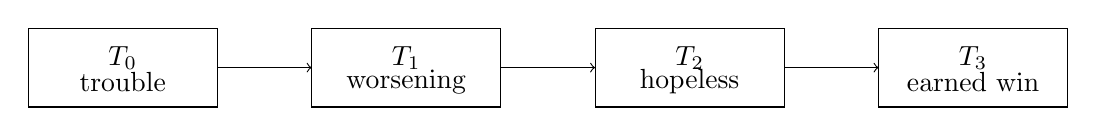
\begin{tikzpicture}
\draw (-1.2,0.5) rectangle (1.2,-0.5);
\node at (0,0.12) {$T_0$};
\node at (0,-0.18) {trouble};

\draw (2.4,0.5) rectangle (4.8,-0.5);
\node at (3.6,0.12) {$T_1$};
\node at (3.6,-0.18) {worsening};

\draw (6.0,0.5) rectangle (8.4,-0.5);
\node at (7.2,0.12) {$T_2$};
\node at (7.2,-0.18) {hopeless};

\draw (9.6,0.5) rectangle (12.0,-0.5);
\node at (10.8,0.12) {$T_3$};
\node at (10.8,-0.18) {earned win};

\draw[->] (1.2,0) -- (2.4,0);
\draw[->] (4.8,0) -- (6.0,0);
\draw[->] (8.4,0) -- (9.6,0);
\end{tikzpicture}
\end{figure}

This diagram is only a transcript-backed reconstruction, but it captures the explicit sequence Jenkins names. It also explains why he places structure before the later discussion of openings, characters, and escalation. The novel needs a carrying chain before it can be ornamented or sharpened.

\section{Character, Research, and Point of View}

The lecture next turns from the engine to the carriers of the engine. A protagonist is not merely a placeholder for events. Jenkins insists that the lead character must have an arc: by the end, he must be a different, preferably better, person. That change is not decorative. It is the very condition under which the late victory can feel earned rather than accidental.

At the same time the antagonist must not be a cardboard villain. Jenkins is precise about the mistake to avoid: the bad guy is not to be evil merely because the plot needs one. He should have motives he can believe in. In that sense the lecture asks for symmetry of seriousness: the opposing force must be as compelling, within its own logic, as the hero.

The same pressure is applied to secondary characters. Jenkins mentions a larger list of questions for developing them, but the transcript is corrupted at that point. What survives clearly is the advice that names, initials, appearances, and voices should be distinct enough that readers do not confuse one character with another. The point is not trivia. Narrative clarity depends on recognizability.

A second inner-outer structure now appears. The lead character faces an outward problem, but he becomes alive on the page through inward turmoil. The external goal and the internal weakness must be brought into contact.

The lecture then pivots to research. Fiction is made up, but it must still be believable. Even fantasy and science fiction must cohere enough to preserve willing suspension of disbelief. Jenkins gives us a compact ratio here:

\begin{equation}
\text{Research}=\text{flavor},\qquad \text{Story}=\text{main course}.
\end{equation}

That is an unusually good formula. It preserves both halves of the problem. Without factual or internally consistent detail, the story loses credibility; with too much accumulated fact, the story is buried under its own seasoning.

The next move is point of view. Jenkins treats this not as a decorative choice of grammatical person alone, but as a bound on narrative information. Who serves as the story's camera? That question determines what can legitimately appear on the page.

We can summarize the rule schematically by letting \(s\) denote a scene and \(\mathrm{POV}(s)\) its viewpoint character:

\begin{equation}
|\mathrm{POV}(s)|=1.
\end{equation}

Jenkins himself states the rule in prose: one perspective character per scene, with his own stricter preference being one per chapter and, ideally, one per novel. Once that bound is fixed, the information channel narrows:

\begin{equation}
\mathrm{Info}(s)=\{\text{see, hear, touch, smell, taste, think}\}_{\mathrm{POV}(s)}.
\end{equation}

This is not lecture-visible notation, but it says exactly what Jenkins says in words. The narrative may carry what the viewpoint character perceives and thinks. We are in that character's mind, employing that character's senses and emotions. From there the lecture resolves a common confusion: this restriction does not force us into first person. Third person limited is perfectly compatible with a single information channel, and in fact it is the dominant modern form. What Jenkins rejects is loose omniscience, the old habit of slipping casually in and out of multiple minds within the same scene.

\subsection{Question \& Answer}

\paragraph{Question.} How does point of view constrain what the novel can reveal?

\paragraph{Answer.} Point of view is an information boundary. Once we choose the perspective character for a scene, the prose is limited to what that character can perceive, infer, remember, and think. We may still reveal a great deal, but we reveal it through the pressure of one consciousness at a time.

\section{Beginning in the Midst of Things and Triggering the Reader's Mind}

Only after all this groundwork does Jenkins reach the opening proper. That order is correct. We first need a project, a structure, a cast, and a viewpoint boundary; only then can we ask how the novel should begin.

His headline term is classical and exact: begin \emph{in medias res}, in the midst of things. He immediately clarifies the usual misunderstanding. This does not necessarily mean bullets flying or a chase scene. It means that we do not waste the opening in inert scene-setting or explanation. The prose must enter where something is already at stake.

That principle can be written as a local rule of motion:

\begin{equation}
\text{sentence } n \Rightarrow \text{desire to read sentence } n+1.
\end{equation}

Jenkins then offers four kinds of opening line: the surprise opener, the dramatic statement, the philosophical opener, and the poetic opener. The lecture's examples are well chosen because they demonstrate different ways to produce forward pull. We do not need to reduce them to a single recipe. We only need to see why each of them compels a continuation. A clock striking \(13\) is a disturbance in the world. A sudden shooting is a disturbance in action. A sweeping maxim about families is a disturbance in thought. A strange, vivid, slightly comic image is a disturbance in tone and expectation.

But the lecture is careful not to let the opening become a fetish. A strong first line is not enough. Many novels begin well and then immediately fall back into explanation. So Jenkins pushes us forward into the next beat: the theater of the reader's mind.

His claim is strong. The task is not to force the reader to see exactly what we see, but to trigger the reader's own imaginative construction. We do that by giving evidence and letting the mind work. This is why the lecture now pivots into the distinction between telling and showing:

\begin{equation}
\text{Telling} \Rightarrow \text{reader is informed},\qquad
\text{Showing} \Rightarrow \text{reader deduces}.
\end{equation}

\subsection{Question \& Answer}

\paragraph{Question.} What does it really mean to show rather than tell?

\paragraph{Answer.} It means that we replace abstract report with observable evidence. Instead of directly asserting the hidden state, we present the cues from which the reader can infer that state. The reader is not merely receiving information; the reader is participating in the construction of meaning.

\paragraph{A worked update rule.} Jenkins's examples can be formalized as a four-step conversion:

\begin{enumerate}
\item Identify the abstract report: tall, angry, cold, frightened, and so on.
\item Ask what the reader could actually witness on the page.
\item Replace the abstract predicate with visible or audible evidence.
\item Remove the redundant direct statement once the evidence carries the meaning.
\end{enumerate}

The lecture gives us two clean examples:

\begin{align}
\text{``He was tall.''} &\to \text{others look up at him; he ducks through a doorway},\\
\text{``He was angry.''} &\to \text{his face flushes, his throat tightens, his voice rises, his fist strikes the table}.
\end{align}

In both cases the abstract predicate is replaced by evidence. The reader performs the last step internally.

\section{Escalation, the Bleakest Moment, and the Difference Between Climax and Ending}

By the time Jenkins reaches step eight, the lecture has prepared us for escalation. We have already seen the Koontz sequence in abstract form. Now it returns with flesh on it. The protagonist has been plunged into trouble; the next task is to make every attempt to escape increase the pressure rather than relieve it.

This is where Jenkins states the strongest maxim of the lecture:

\begin{equation}
\text{Conflict}=\text{engine of fiction}.
\end{equation}

He makes the point by negative example. Too many beginners give the hero everything: good looks, health, good equipment, money, a useful client, a supportive domestic life. That is the architecture of comfort, not of narrative. Jenkins's corrective is simple and severe: strip supports away. Remove ease. Make the case poorer, the body weaker, the marriage unstable, the tools unreliable, the office gone. Once enough supports have been removed, the story begins.

We can now write the late narrative chain in the form in which the lecture actually uses it:

\begin{equation}
\text{trouble} \to \text{worsening trouble} \to \text{bleakest moment} \to \text{climax} \to \text{ending}.
\end{equation}

The new named object here is the bleakest moment, Angela Hunt's term for the point at which even the writer wonders how the story can possibly be repaired.

\begin{definition}
The bleakest moment is the local nadir of the plot, the point at which the protagonist's predicament appears beyond repair.
\end{definition}

Jenkins is emphatic that we must not cheat here. No easy escape. No artificial break. No miracle inserted merely because the writer has become afraid of the consequences of the structure.

\subsection{Question \& Answer}

\paragraph{Question.} How hopeless should the hero's situation become before the ending can feel earned?

\paragraph{Answer.} Hopeless enough that both reader and writer can no longer see an easy path out. The point of the bleakest moment is precisely to force the protagonist to act with everything the novel has built into him. If the crisis is softened too soon, the ending loses force.

This leads directly to the next correction. The climax is not the ending.

\begin{equation}
\text{Climax} \neq \text{Ending}.
\end{equation}

The climax is the peak confrontation and the place where the major setups are paid off. The ending comes after that. Its job is different. Jenkins gives two tests for whether the ending is sound:

\begin{itemize}
\item it puts the reader first, honoring the investment of time and attention;
\item it keeps the hero the hero, on stage through the last word.
\end{itemize}

So even after the fireworks of the climax, the novel cannot simply stop. It must still resolve emotionally.

The lecture then closes the loop by returning from narrative structure to writing practice itself. The bonus step is not ornamental. It names a final discipline:

\begin{equation}
\text{Drafting} \neq \text{Editing}.
\end{equation}

Jenkins's advice is to write the first draft with the inner critic muted, then return in a separate mode for revision. That discipline can be summarized as another short procedure:

\begin{enumerate}
\item Draft without stopping for perfection.
\item Let logic gaps, cliches, and roughness remain during the drafting pass.
\item Return later in a distinct revision pass.
\item Fine-tune sentence by sentence only when the drafting motion is over.
\end{enumerate}

The promised twenty-one-part checklist belongs to that later revision phase. Since the transcript does not preserve its contents, we note only its function: it is a separate instrument for refinement, not a tool to be mixed into the first-draft flow.

\section{Summary}

The lecture begins with fear, but it does not stay there. It converts fear into method. We first define the novel as fiction, then choose the one idea whose passion can survive the middle, then distinguish temperament from structure, and then build the story through arc, research, viewpoint, opening pressure, imaginative participation, escalating conflict, the bleakest moment, climax, ending, and revision discipline.

The companion lesson is that even without literal board mathematics, a lecture can have a rigorous structure. Here that structure is procedural. If we compress the whole chapter to one line, it is this: choose the project that can endure, constrain the prose so the reader can enter it, and let the conflict deepen until the ending is truly earned.